%! Suppress = Unicode
%! Author = Adrian Helberg
%! Script = 18.02.2020
%! Presentation = 21.02.2020

%%% Preamble
\documentclass[11pt]{article}

%%% Packages
\usepackage{ngerman}
\usepackage{color} % Colored font
\usepackage{graphicx} % Images
\usepackage{titling} % Title formatting
\usepackage[utf8]{inputenc} % UTF-8
\usepackage {tikz}
\usepackage{amsmath} % Graphs
\usepackage{etoolbox} % Well formatted Links in bib
\apptocmd{\thebibliography}{\raggedright}{}{} % Well formatted Links in bib
\usepackage{hyperref} % Links

%%% Commands
% ToC title
\renewcommand{\contentsname}{
    \begin{center}
        \LARGE Inhalt
    \end{center}
}

%%% Title
\pretitle{
    \begin{center}
        
\includegraphics[width=8cm]{../../resources/Haw_logo.png}
    \end{center}
}
\title{
    \begin{center}
        \Huge \textbf{Intelligente Systeme}\\
        {\color{blue}- Skript -}\\~\\
        \Large Prüfungsform: Referat
    \end{center}
}
\author{Adrian Helberg\\ Matr.Nr. 2309051}
\date{Abgabe: 18.02.2020}

%%% Document
\begin{document}

    \maketitle

    \begin{abstract}
        Diese Arbeit beschäftigt sich mit Konzepten der vier Kernbereiche aus \textit{intelligente
        Systeme}: \textbf{Suchen}, \textbf{Lernen}, \textbf{Verarbeitung von Sequenzen} und
        \textbf{Ethik}. Zum einen werden Problemstellungen aufgezeigt, zum anderen auf
        Implementationen verwiesen, die in der zugehörigen Präsentation vorgestellt werden.\\ Eine
        Lösungsstrategie für das \textit{Problem des Handlungsreisenden (Traveling Salesman
        Problem)} wird im Kapitel \textbf{Suchen} beschrieben~\cite{suchen, salesman, impl}.
        \textit{Selbstorganisierte Karten (Selforganizing Maps)} zeigen eine Strategie des \textbf{Lernen}s~\cite{lernen, som},
        ein \textit{Deep Learning}- Ansatz zur Datenanalyse von Sensordaten mobiler Endgeräte gibt Einblicke in
        die \textbf{Sequenzverarbeitung}~\cite{sequenzen} und eine Diskussion zum \textit{Trolley Problem} lädt
        zur Diskussion über die \textbf{Ethik} in Verbindung mit \textit{intelligenten Systemen}
        ein~\cite{trolley, Eimler2018}.
    \end{abstract}

    \tableofcontents
    \newpage

    \section{Suchen}

    Dieses Kapitel beschäftigt sich mit der Umsetzungen einer Lösungsstrategie für das
    \textit{Problem des Handlungsreisenden (Traveling Salesman Problem)} mithilfe einer
    informierten Suche. Im speziellen eine Umsetzung mit einem genetischen Algorithmus.

    \subsection{Problem des Handlungsreisenden}
    Das Problem des Handlungsreisenden ist ein kombinatorisches Optimierungsproblem der
    theoretischen Informatik. Dabei muss ein Handlungsreisender eine Menge von Städten besuchen.
    Er beginnt bei einer bestimmten Stadt und muss, nachdem jede andere Stadt besucht wurde, zu
    dieser zurückkehren. Das Optimierungsproblem besteht bei der Festlegung der Reihenfolge der zu
    besuchenden Städte, sodass die gesamte Distanz der Reise minimal ist. Das Problem ist als
    NP-vollständig klassifiziert.

    \subsection{Genetischer Algorithmus}
    Evolutionäre Algorithmen sind eine Klasse von stochastischen, heuristischen
    Optimierungsverfahren. Der Name lässt sich von der Evolution natürlicher Lebewesen ableiten.
    Ziel von genetischen Algorithmen ist es optimierte Lösungen zu Aufgabenstellungen zu finden,
    bei denen ein Auffinden einer akzeptablen Lösung aus Gründen der kombinatorischen Komplexität
    misslingt. So gibt es beim Problem des Handlungsreisenden mit 10 Orten z.B. bereits
    $10!=3628800$ Lösungen. Kern eines genetischen Ansatzes ist die Veränderung von Mengen an
    Problemlösungen, sodass gute Lösungen mit einer großen Wahrscheinlichkeit und schlechte
    Lösungen mit geringen Wahrscheinlichkeit erhalten bleiben. Das Zusammenführen von Teilen guter
    Lösungen kann noch bessere Ergebnisse liefern. So kann verhindert werden, dass ein
    Algorithmus zur Optimierung an einem lokalen Optimum "hängenbleibt".

    \newpage

    \subsubsection{Allgemeiner Ablauf}
    \begin{center}
        \begin{tikzpicture}[semithick , state/.style ={ rectangle ,top color =white , bottom color = processblue!20 ,
        draw,processblue , text=blue , minimum width =1 cm}]
            \node[state] (A) at (0,0) {Start};
            \node[state] (B) at (0,-1.2) {Erzeugung einer zufälliger Population};
            \node[state] (C) at (0,-2.4) {Wiederhole bis Abbruchbedungung erfüllt};
            \node[state] (D) at (0,-3.6) {Berechne Fitness};
            \node[state] (E) at (0,-4.8) {Selektion};
            \node[state] (F) at (0,-6) {Crossover};
            \node[state] (G) at (0,-7.2) {Mutation};
            \node[state] (H) at (0,-8.4) {Austausch};
            \node[state] (I) at (0,-9.6) {Teste Abbruchbedingung};
            \node[state] (J) at (0,-10.8) {Ende};

            \draw[->, very thick] (A) to (B);
            \draw[->, very thick] (B) to (C);
            \draw[->, very thick] (C) to (D);
            \draw[->, very thick] (D) to (E);
            \draw[->, very thick] (E) to (F);
            \draw[->, very thick] (F) to (G);
            \draw[->, very thick] (G) to (H);
            \draw[->, very thick] (H) to (I);
            \draw[->, very thick] (I) to (J);
        \end{tikzpicture}
    \end{center}

    \subsection{Chromosomen}
    Eine Rundreise des \textit{Handlungsreisenden} wird duch ein Chromosom repräsentiert. Er
    bereist hierzu alle Städte und endet in der Stadt, in der begonnen hat. Die Population
    besteht aus der Anzahl solcher Rundreisen, die durch Vektoren modelliert werden.\\
    Eine mögliche Rundreise wäre also:
    \left\{
    \begin{array}{c}
        3\\5\\1\\2\\4\\3
    \end{array}
    \right\}

    \subsection{Fitness}
    Eine Berechnung der Fitness in Abhängigkeit von der Gesamtdistanz einer Rundreise bietet sich
    für das \textit{Problem des Handlungsreisenden} an. Allerding soll der Fitness-Wert
    proportional zur Eignung (antiproportional zu den Kosten) eines Chromosoms sein. Für die
    Kosten wird die Gesamtdistanz eines Chromosoms, für die Fitness der inverse Kostenwert
    verwendet.

    \subsection{Selektion}
    Die Auswahl eines Chromosomenpaars aus der Population soll wahrscheinlicher werden, wenn der
    Fitness-Wert steigt. Dies kann mittels einer Summe über alle Fitness-Werte gleichverteilte
    Zufallszahl realisiert werden. Der Wertebereich der Zufallszahl wird in Abschnitte
    unterteilt, deren Größe genau den Fitnesswerten der einzelnen Chromosomen entsprechen. Der
    Abschnitt, in den die Zufallszahl fällt, bestimmt die Selektion des zugehörigen Chromosoms.

    \subsection{Kreuzung}
    Ein zufälliger Kreuzungspunkt innerhalb des Vektors eines selektierten Chromosoms wird bestimmt.
    Der neue Vektor ist bis zum Kreuzpunkt identisch mit dem ursprünglichen. Der restliche Teil
    des neuen Vektors wird wie folgt bestimmt. Gehe den zweiten ausgewählten Vektor vom Anfang
    bis zum Ende durch und füge die erste Zahl, die noch nicht im neu zu bildenden Chromosoms
    steht, an die nächste freie Stelle ein. An der letzten Stelle des neuen Chromosomes muss die
    gleiche Zahl stehen wie an seiner ersten Stelle. Dieser Prozess wird für beide ausgewählten
    Chromosomen durchgeführt.

    \subsection{Mutation}
    Mit einer kleinen Wahrscheinlichkeit findet in der Kreuzung eine Mutation statt. Diese wird
    wie folgt implementiert. Ein zufälliges Paar von Indizes mit Werten zwischen 1 und der Anzahl
    der Städte wird erzeugt. Die Werte, die den Indizes entsprechenm werden im Chromosom getauscht.
    Dabei darf die Eigenschaft, dass Start- und Zielwert identisch sind, nicht verletzt werden.

    \subsection{Austausch}
    In jeder Iteration werden in der Population die beiden schlechtesten Chromosomen, d.h.
    diejenigen mit den geringsten Fitness-Werten, durch die beiden neuen Chromosomen ersetzt, falls
    letztere bessere Fitness-Werte haben. Es wird gewährleistet, dass in der Population alle
    Chromosomen verschieden sind.

    \subsection{Realisierung mit Java}

    \subsubsection{Eigenschaften}
    \begin{center}
        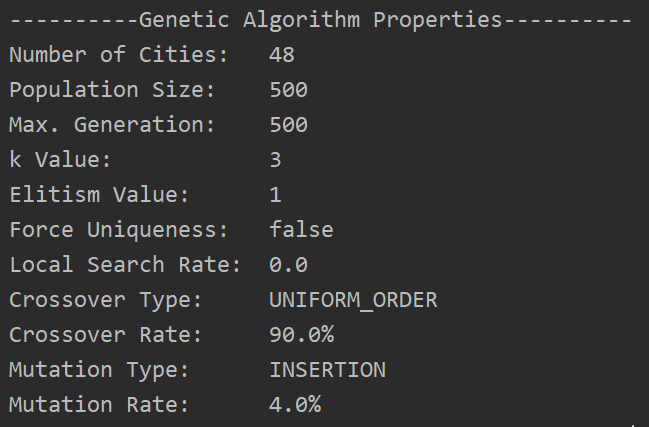
\includegraphics[width=10cm]{../../resources/properties_algorithm.png}
        \\~\\
        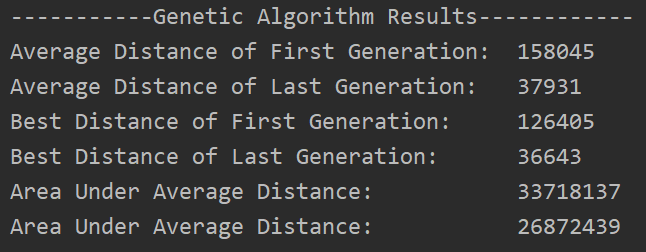
\includegraphics[width=10cm]{../../resources/properties_results.png}
    \end{center}

    \subsubsection{Visualisierung}

    \begin{center}
        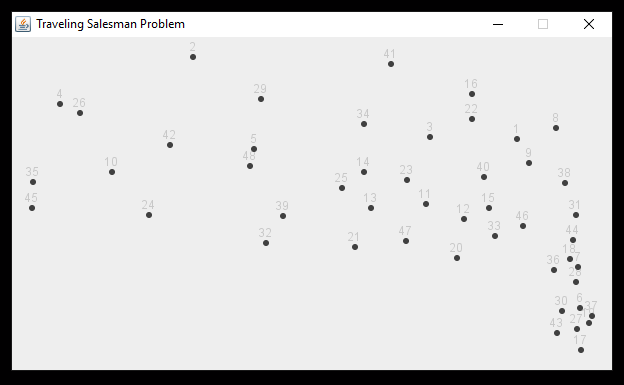
\includegraphics[width=10cm]{../../resources/tsp_cities.png}
        \\~\\
        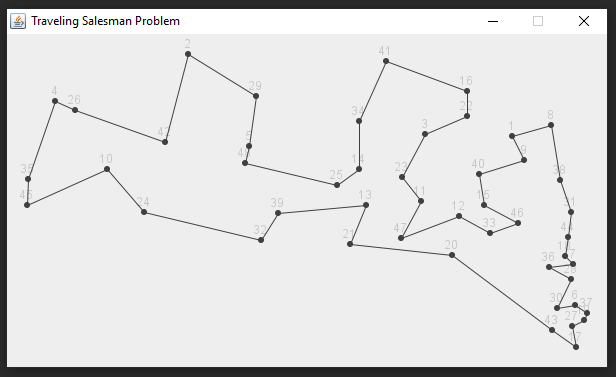
\includegraphics[width=10cm]{../../resources/tsp_cities_connected.png}
    \end{center}

    \newpage

    \section{Lernen}

    Dieses Kapitel beschreibt ein unüberwachtes Lernverfahren der Neuroinformatik: Die
    \textit{Selbstorganisierenden Karten}, \textit{Kohonen-Karten}, oder \textit{Kohonen Feature
    Maps}. Also maschinelles Lernen ohne oder vorher bekannte Ergebniswerte.

    \subsection{Motivation}
    Das Funktionsprinzip von \textit{SOM}s (\textit{Self-organizing maps}) beruht auf der
    Erkenntnis, dass viele Strukturen im Gehirn eine lineare oder planare Topologie aufweisen.
    Eingehende Signale, wie z.B. visuelle Reize, sind jedoch multidimensional. Abbildung 1 zeigt
    eine Skizze der topologischen Ansicht des sensorischen Kotex, der die sensorischen Eingaben
    des Körpers auswertet. Es entsteht eine Klassifizierung, da ähnliche Ausgaben in direkter
    Umgebung angesiedelt werden. Beispielsweise sind Signale an die Finger in unmittelbarer
    Nachbarschaft zueinander. Solch eine Nachbarschaftsbeziehung zwischen Neuronen ist ein
    grundlegendes Merkmal von \textit{SOM}s

    \begin{figure}[ht!]
        \centering
        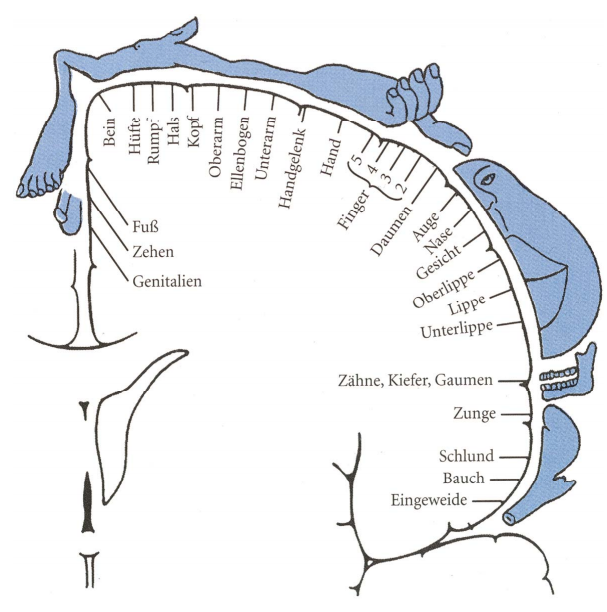
\includegraphics[width=8cm]{../../resources/gehirn.png}
        \caption{Topologische Abbildung des sensorischen Kortex}
    \end{figure}
    \newpage

    Eine topologieerhaltende Abbildung auf weniger Dimensionen (siehe Kapitel
    \textbf{Motivation}), hier eine Fläche, wird als Karte bezeichnet. Diese Karten im Gehirn
    kommen bei allen Säugetieren vor und sind dynamisch. Dies wird an folgendem Beispiel deutlich.
    Beim Verlust von Körperteilen wird der Platz des entsprechenden Feldes mit der Zeit von
    anderen Feldern eingenommen (da die eingehenden Signale wegfallen, Abbildung 2).

    \begin{figure}[ht!]
        \centering
        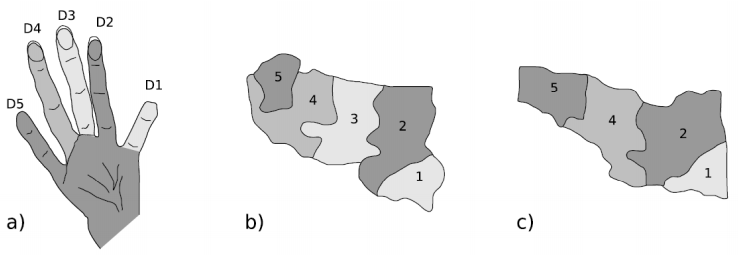
\includegraphics[width=12cm]{../../resources/aufbau.png}
        \caption{a) Schema einer Affenhand b) Bereich des Kortex der Hand c) 2 Monate nach
        Amputation von Finger D3}
    \end{figure}

    \subsection{Aufbau}
    \textit{SOM}s verwenden ein sehr einfaches Neuronenmodell ohne Aktivierungsfunktion
    (Abbildung 3)

    \begin{figure}[ht!]
        \centering
        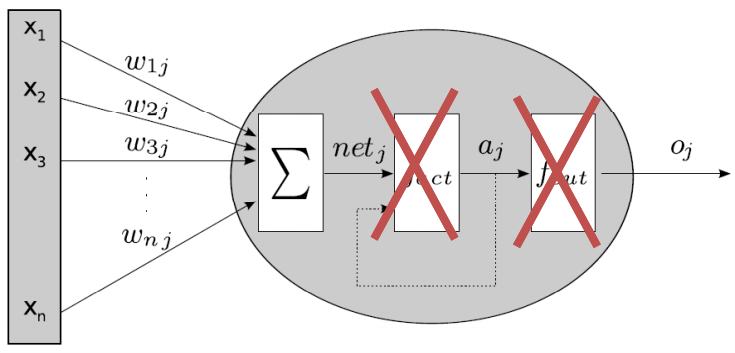
\includegraphics[width=12cm]{../../resources/neuron.png}
        \caption{Neuron einer \textit{SOM}}
    \end{figure}

    \subsection{Netz}
    Organisiert man Neuronen als Eingabe- und Ausgabeneuronen in jeweils einer
    Schicht, entsteht ein neuronales Netz, in dem die Eingabeneuronen über die Gewichtsvektoren
    komplett mit den Ausgabeneuronen verbunden sind (Abbildung 4).

    \begin{figure}[ht!]
        \centering
        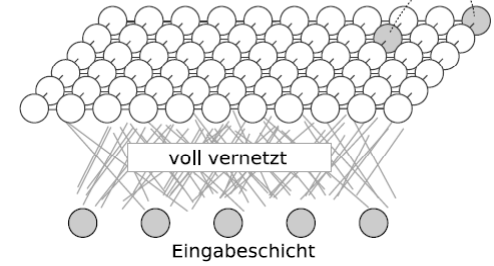
\includegraphics[width=12cm]{../../resources/netz.png}
        \caption{\textit{Kohonen}-Netz}
    \end{figure}

    \subsection{Lernverfahren}
    \textit{SOM}s lernen durch Auswahl eines Neurons anhand deren "`Eignung"'. Die Eignung wird
    über die euklidische Norm berechnet. Hierbei wird der Abstand zwischen Eingabevektor und
    Gewichtsvektor bestimmt. Besitzen Neuronen die gleiche euklidische Norm, wird über das
    Zufallsprinzip entschieden, welches Neuron ausgewählt wird. Das Besondere an \textit{SOM}s
    ist, dass nicht nur der Gewichtsvektor des ausgewählten Neurons (Siegerneuron) verändert
    wird, sondern auch die der Neuronen in der Umgebung des Siegerneurons.
    \newpage

    \subsection{Distanzfunktion}
    Anstelle der euklidischen Norm werden in der Praxis auch andere bewährte Distanzfunktionen
    verwendet. Einige Beispiele sind die gaussche Glockenfunktion, die Zylinderfunktion und der
    "`Mexican-Hat"' (Abbildung 5).

    \begin{figure}[ht!]
        \centering
        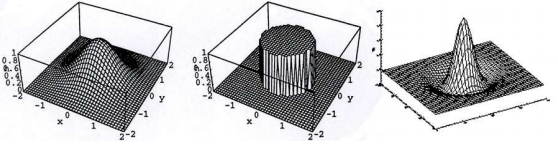
\includegraphics[width=12cm]{../../resources/distanzfunktionen.png}
        \caption{Gaussche Glockenfunktion, Zylinderfunktion und Mexican-Hat}
    \end{figure}


    \subsection{Siegerneuron anpassen}
    \begin{center}
        $W_c = W_c + \Delta W_c$ und $\Delta W_c = \eta * (x-W_c)$
    \end{center}
    Mit $c$ als Siegerneuron, $W_c$ als Gewichtungsvektor und Eingabevektor $x$.\\
    Es gilt $0 < \eta < 1$.


    \subsection{Nachbarneuronen des Siegerneurons anpassen}
    Nachbarn des Siegerneurons lernen umso stärker, je näher sie sich am Siegerneuron befinden:
    \begin{center}
        $\Delta W_j = \eta * h_c_j * (x - W_j)$
    \end{center}
    Mit $h_c_j$ als Nachbarschaftsfunktion (Wie stark lernt das Neuron $j$ mit bei Siegerneuron $c$)\\
    Als Funktion des Abstandes $z$ der Neuronen wird in der Praxis oft eine Zylinderfunktion gewählt:
    \begin{center}
        $Zylinder: h_c_j(z) =
        \begin{cases}
            1 & falls \; z < d\\
            0 & sonst.
        \end{cases}$
    \end{center}

    \newpage

    \subsection{Visualisierung}
    \begin{figure}[ht!]
        \centering
        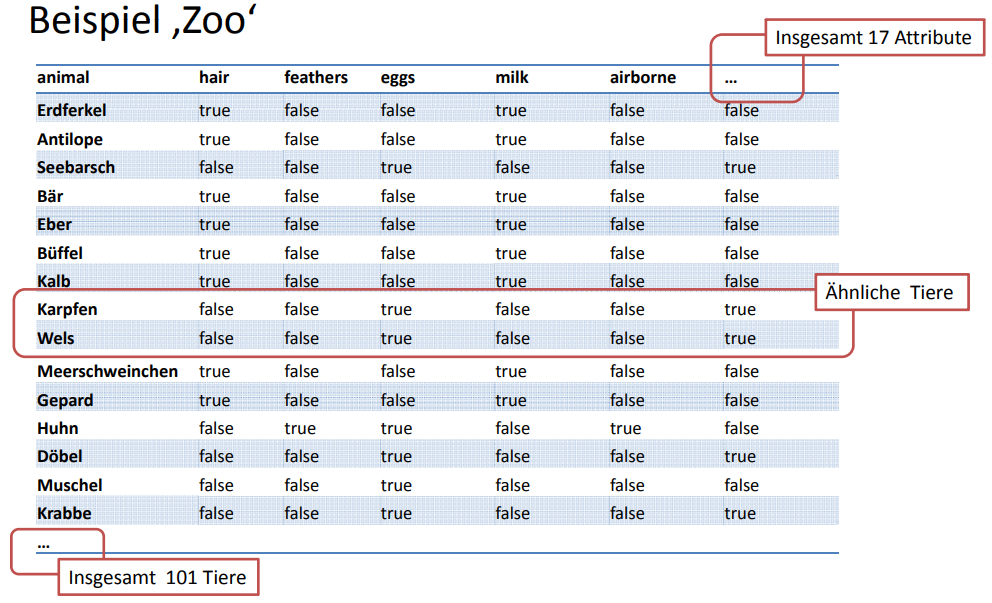
\includegraphics[width=15cm]{../../resources/zoo_table.png}
        \caption{Beispiel "`Zoo"'}
    \end{figure}

    \begin{figure}[ht!]
        \centering
        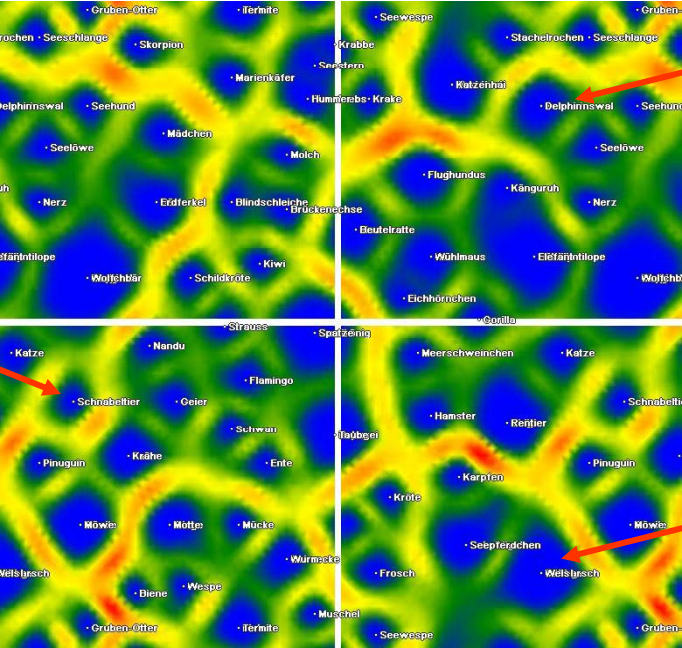
\includegraphics[width=12cm]{../../resources/zoo.png}
        \caption{Beispiel "`Zoo"'}
    \end{figure}
    Reduktion von mehreren Dimension auf 2 (Karte). Sind ähnliche Tiere eines Zoos benachbart?
    (Abbildung 6+7)
    \newpage

    \subsection{Anwendungsgebiete}
    \begin{itemize}
        \item Dimensionsreduktion
        \item Optimierung
        \item Data Mining- Cluster
        \item Data Mining - Regeln
        \item Überwachenung und Anomaliedetektion
        \item Kontextkarten
    \end{itemize}

    \section{Sequenzen}
    Die Verarbeitung von Sensordaten mobiler Endgeräte (z.B. Smartphones) wird in diesem Kapitel
    vorgestellt. Hierzu wird ein \textit{Deep Learning} Ansatz gewählt.

    \subsection{Motivation}
    Die zunehmende Beliebtheit tragbarer Endgeräte der letzten Jahre
    gibt die Möglichkeit eine Vielzahl von physiologischen und funktionellen Daten kontinuierlich
    zu erfassen. Diese können Anwendungen für Sport, Gesundheit und Wohlbefinden zur Verfügung
    gestellt werden. Die Masse an Informationen erfordert effiziente Klassifizierungsmethoden und
    sinnvolle Analyse, wobei ein \textit{Deep Learning} Ansatz eine vielversprechende Technik für
    die Datenanalyse im großen Stil ist. Die \textit{Human Activity Recognition} (HAR) wertet
    zeiliche Reihendaten von Trägheitssensoren aus, um eine Aktion  identifizieren
    zu können, die ausgeführt wird. So kann sowohl einen Ausbruch von Krankheiten (z.B. Parkinson),
    als auch die Wirksamkeit einer Behandlung erkannt werden.

    \subsection{Problem}
    Während \textit{Deep Learning} bei Implementationen, die Hochleistungs-Rechencluster nutzen,
    bisher sehr erfolgreich war, ist der Einsatz auf mobilen Endgeräten durch geringe Ressourcen
    beschränkt.

    \subsection{Technik}
    Eine der größten Herausforderungen beim Entwerfen einer Klassifizierungsmethode für eine
    Zeitreihenanalyse ist die Auswahl von Merkmalen der Klassen. Oft kann durch den Einsatz
    von \textit{Deep Believe Networks} (DBN), \textit{Restricted Boltzman Machines} (RBM) oder
    \textit{Convolutional Neural Networks} (CNN) eine Menge von \textit{Features} (Markmale) der
    Rohdaten herausgearbeitet werden. Um eine vollständige Hierarchie der Features herauszufinden,
    die die Rohdaten sinnvoll klassifizieren kann, wird bei \textit{HAR} jedoch ein
    \textit{Deep Learnung} Ansatz mit komplexen Designs und vielen Schichten benötigt, um Änderungen
    in den verschiedenen Sensoren verarbeiten zu können.
    \newpage

    \subsection{"`Shallow Deep Learning"' Methode}
    Im folgenden werden die einzelnen Schritte der vorgeschlagenen Methode gezeigt. Diese setzt
    sich aus \textit{Deep Learning} (Prozess A) und \textit{Shallow Learning} (Prozess B) zusammen.

    \begin{figure}[ht!]
        \centerings
        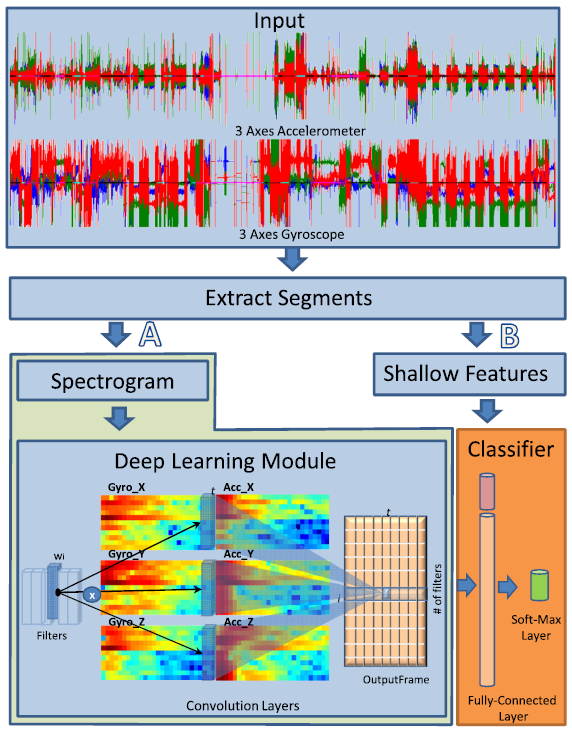
\includegraphics[width=12cm]{../../resources/prozess.png}
        \caption{Schematischer Ablauf der Methode}
    \end{figure}

    \subsubsection{Input}
    Um eingehende Daten (Input) zu generieren, wird auf verbaute Trägheitssensoren wie
    Beschleunigungsmesser und Gyroskope zugegriffen. Das Nutzen von Zeitreihendaten von anderen
    Sensoren, wie Elektrokardiographie (EKG) oder Elektromyographie (EMG), sind
    ebenfalls möglich.

    \subsubsection{Segmente extrahieren}
    Nachdem die Rohdaten eingesammelt werden, können $n$ Segmente extrahiert werden, wobei $n$
    von der Art der Applikation abhängt. Die Länge der Segmente wird bei \textit{HAR} auf
    4 bis 10 Sekunden (\textit{sliding window}) gesetzt, um die Genauigkeit der Erkennung der
    ausgeführten Aktivität zu maximieren, ohne die Grenzen zwischen verschiedenen Aktivitäten
    zu verschleiern.

    \subsubsection{Spektogramm und Deep Learning Modul}
    Um nun \textit{Features} zu extrahieren, werden die Segmente als Spektogramm-Repräsentation
    an ein \textit{Deep Learning} Modul weitergereicht, das darauf ausgelegt ist
    Intensitätsunterschiede in den Trägheitspunkten des Spektogramms zu interpretieren. Die Zeit-
    und Abtastrateninvarianz, die Amplituden und die Frequenz kann zur Untersuchung der Spektogramme
    genutzt werden (z.B. durch \textit{Fourier}-Transformation).\\
    Es ergeben sich beispielsweise folgende \textit{Features}: (Abbildung 9)

    \begin{figure}[ht!]
        \centerings
        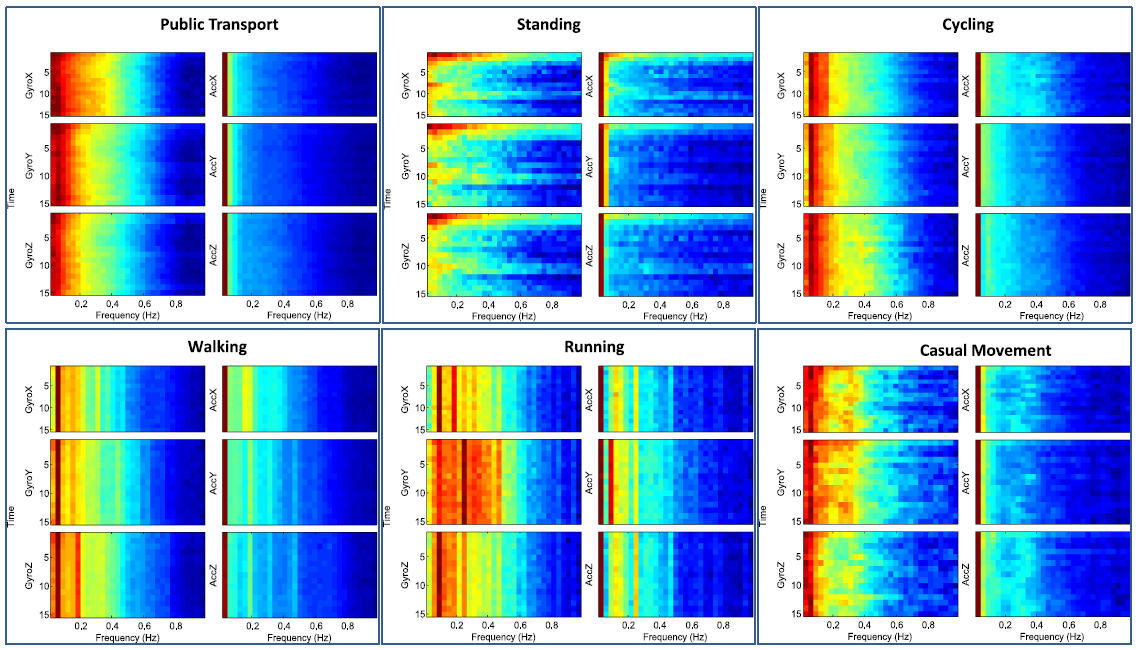
\includegraphics[width=11.8cm]{../../resources/features.png}
        \caption{Spektogramme aus verschiedenen Aktivitäten}
    \end{figure}

    \subsubsection{Shallow Features}
    Aus verschiedenen Berechnungen ("`flache"' Merkmale), die auf die Spektogramme angewendet werden
    (z.B. Quadratischer Mittelwert, Standartabweichung, usw.), kann nun eine Vektorrepräsentation
    jedes Segments erstellt werden.

    \subsubsection{Klassifizierung}
    Sobald sowohl flache (\textit{shallow learned}), als auch tiefe (\textit{deep learned})
    Eigenschaften berechnet wurden, können diese zu einem eindeutigen Vektor zusammengeführt und
    klassifiziert werden.

    \subsubsection{Training}
    Flache und tiefe Features werden zusammen in einem einheitlichen, neuronalem Netz trainiert. In
    jeder Schicht des neuronalen Netzes werden Fehler (Errors) zwischen den Soll- und Istwerten in
    einer \textit{Backwards Propagation} Routine genutzt, um die Gewichtungen in den
    \textit{Hidden-Layers} anzupassen.

    \subsection{Evaluation (Vorschlag)}
    Das vorgeschlagene \textit{Shallow Deep Learning}-Verfahren könnte nun mit verschiedenen Datensätzen
    (Abbildung 10) analysiert und evaluiert werden.

    \begin{figure}[ht!]
        \centerings
        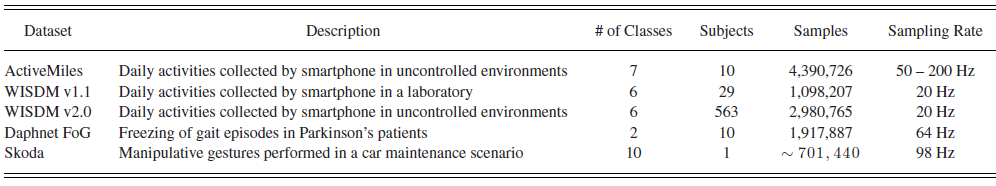
\includegraphics[width=16cm]{../../resources/datasets.png}
        \caption{Datensätze für eine Evaluierung}
    \end{figure}

    \newpage

    \section{Ethik}

    \subsection{Thema}

    \subsection{Verantwortung als Informatiker}

    \newpage

    \bibliographystyle{plain}
    \bibliography{script}

\end{document}